% !TeX program = pdflatex
% =============================================================================
% Arbeitsblatt: Magnetfelder
% UZH Praktikum I -- Sara Romer Urban, Kantonsschule im Lee, HS2026
% Klasse: 4fh (01.09.2026, nur 4fh -- 4cdeg hat hier Hospitation, kein
% eigenes Dokument noetig).
%
% Ablauf (direkt mit Loris per Chat abgestimmt, 31.08.2026 -- ersetzt die
% Reihenfolge aus einer frueheren Fassung dieser Datei):
%   1. Repetition Magnete/Kompassnadel (Werkstatt-Quiz + Bildfrage zum
%      Kompassverhalten in Naehe eines Magneten -- Bild folgt von Loris).
%   2. Vergleich elektrisches Punktladungsfeld vs. Stabmagnetfeld (Bilder
%      folgen von Loris).
%   3. Regeln zum Zeichnen von Feldlinien + Zeichenuebung (zwei Stabmagnete,
%      gleichnamige Pole zueinander).
%   4. Erdmagnetfeld.
%   5. Oersted-Geschichte (kurz, als Ueberleitung).
%   6. Baukasten-Experiment (Partnerarbeit): Stromkreis mit Stableiter und
%      Spule, Feld mit kleinen Kompassnadeln erkunden, danach Stromrichtung
%      umkehren -- bewusst VOR der Theorie (entdeckendes Lernen).
%   7. Theorie: Rechte-Faust-Regel + Formeln fuer geraden Leiter und Spule.
%   8. Ein paar Aufgaben (Formelanwendung).
%
% Ring/Helmholtz-Spule, Ringspule (Toroid) und die Permeabilitaets-
% Sortieraufgabe sind auf Loris' ausdruecklichen Wunsch NICHT mehr Teil
% dieser Doppellektion (Stand 31.08.2026) -- lernziele.md (LZ3/LZ4) und
% magnetfelder-lektionsplan.tex sind entsprechend VERALTET und muessen noch
% separat nachgezogen werden, bevor sie wieder als Quelle fuer dieses
% Dokument gelten.
%
% Noch keine eigenen Skizzen fuer die neuen Abschnitte (Kompass-Bild,
% Punktladungsfeld/Stabmagnetfeld-Vergleich, Erdmagnetfeld) -- echte Bilder
% folgen, sobald sie vorliegen; bis dahin bewusst nur Text (siehe
% TODO-Kommentare im Fliesstext). leiter.png/spule.png sind bereits
% vorhanden und werden weiterhin verwendet.
%
% Quellen: Vorwissen/Magnetismus/Werkstatt_Magnetismus.docx
% (15-Posten-Werkstatt, bereits bekannt), PhysikLibre Kap. 13.1/13.4 (dieser
% Ordner), LEIFIphysik (Magnetfeld gerader Leiter/Zylinderspule).
% =============================================================================
\documentclass[addpoints,11pt,a4paper]{exam}

\usepackage[T1]{fontenc}
\usepackage[utf8]{inputenc}
\usepackage[ngerman]{babel}
\usepackage{lmodern}
\usepackage[a4paper,margin=2.2cm,headheight=14pt]{geometry}
\usepackage{amsmath}
\usepackage{amssymb}
\usepackage{siunitx}
% Hausstil: zusammengesetzte Einheiten immer als echter Bruch (\frac), nicht
% als Inline-Schrägstrich oder \tfrac -- gilt global für jedes \si/\SI.
\sisetup{per-mode=fraction,fraction-command=\frac}
\usepackage{array,booktabs,tabularx,multirow}
\usepackage{enumitem}
\usepackage{xcolor}
\usepackage{colortbl}
\usepackage{tikz}
\usepackage{physics}
\usepackage{circuitikz}
\usepackage[most]{tcolorbox}
\usepackage{lastpage}
\usepackage{graphicx}
\usepackage{hyperref}

\usetikzlibrary{arrows.meta,calc,angles,quotes,decorations.markings}

\usepackage{setspace}
\usepackage{needspace}
\setlength{\parindent}{0pt}
\setlength{\parskip}{0.6em}
\setstretch{1.08}
\setlist[itemize]{itemsep=0.4em}

% -----------------------------
% Farben (Corporate-Farbschema Physik KFR)
% -----------------------------
\definecolor{titleblue}{HTML}{183A6B}
\definecolor{accentblue}{HTML}{2E6F9E}
\definecolor{lightblue}{HTML}{EAF4FB}
\definecolor{verylightblue}{HTML}{F7FBFE}
\definecolor{lightgray}{HTML}{F4F6F8}
\definecolor{darkgray}{HTML}{4A4A4A}
\definecolor{accentorange}{HTML}{D9720C}
\definecolor{accentpurple}{HTML}{7B2D8E}
% Theorie-Block: eigene Farbe (grün).
\definecolor{theorygreen}{HTML}{2E7D4F}
\definecolor{lighttheorygreen}{HTML}{EAF7EF}
% Gruppenarbeit-Box: eigene Farbe (Petrol/Teal).
\definecolor{groupteal}{HTML}{1B7F72}
\definecolor{lightgroupteal}{HTML}{E8F5F3}
% Hinweisbox: Orange (accentorange), für wichtige Klarstellungen.
\definecolor{lightorange}{HTML}{FCEEE0}
% Formelbox: Violett (accentpurple), für die zentralen Formeln dieser Einheit.
\definecolor{lightpurple}{HTML}{F3EAF7}

% Links (hyperref): farblich ans Corporate-Farbschema angeglichen.
\hypersetup{
  colorlinks=true,
  urlcolor=accentblue,
  linkcolor=accentblue,
  pdftitle={Arbeitsblatt 5: Magnetfelder},
  pdfauthor={Loris Keller}
}

% -----------------------------
% Spaltentypen
% -----------------------------
\newcolumntype{Y}{>{\centering\arraybackslash}X}
\newcolumntype{P}[1]{>{\raggedright\arraybackslash}p{#1}}

% -----------------------------
% Boxen
% -----------------------------
\tcbset{before skip=10pt, after skip=10pt}
\newtcolorbox{titlebox}{
  enhanced,
  colback=titleblue,
  colframe=titleblue,
  boxrule=0pt,
  arc=3mm,
  left=3mm,right=3mm,top=3mm,bottom=3mm
}

\newlength{\aufgabenindent}
\settowidth{\aufgabenindent}{10.\hskip\labelsep}

% Praktikum I: Lernziele/Einleitung/Theorie/Aufgaben werden NICHT mehr
% farbig gerahmt (nur Formel-, Hinweis- und Antwortbox bleiben Boxen) --
% siehe institutionen/UZH-Praktikum-I/CLAUDE.md, Abschnitt "Boxen-Layout".
\newenvironment{infobox}{%
  \par\addvspace{10pt}\noindent
}{%
  \par\addvspace{10pt}
}

\newenvironment{theoriebox}[1][Theorie]{%
  \par\addvspace{10pt}\noindent\textbf{#1}\par\smallskip\noindent
}{%
  \par\addvspace{10pt}
}

% taskbox/groupbox stehen in questions VOR dem ersten \question (Bilder,
% Fliesstext) -- exam.cls' questions-Liste braucht dafür eine echte,
% eigenständige Box (sonst "Something's wrong--perhaps a missing \item",
% weil z.B. ein \begin{center} vor dem ersten \item der Aussenliste steht).
% Deshalb bleiben es tcolorboxen, nur unsichtbar gemacht (keine Farbe/Rahmen,
% kein Padding) statt sie durch reine Absätze zu ersetzen.
\newtcolorbox{taskbox}[1][]{
  enhanced, breakable,
  colback=white, colframe=white, boxrule=0pt,
  left=0mm,right=0mm,top=0mm,bottom=0mm,
  before skip=10pt, after skip=10pt,
  before upper={%
    \def\tmpboxtitle{#1}%
    \ifx\tmpboxtitle\empty\else\noindent\textbf{#1}\par\smallskip\fi
  }
}

\newtcolorbox{groupbox}[1][Gruppenarbeit]{
  enhanced, breakable,
  colback=white, colframe=white, boxrule=0pt,
  left=0mm,right=0mm,top=0mm,bottom=0mm,
  before skip=10pt, after skip=10pt,
  before upper={\noindent\textbf{#1}\par\smallskip}
}

% beispielbox: für die Einleitung und für durchgerechnete Beispiele
% innerhalb der Theorie -- wie die anderen Inhaltsboxen ungerahmt.
\newenvironment{beispielbox}[1][Beispiel]{%
  \par\addvspace{10pt}\noindent\textbf{#1}\par\smallskip\noindent
}{%
  \par\addvspace{10pt}
}

% hinweisbox: Orange, für wichtige Klarstellungen/Verwechslungswarnungen.
\newtcolorbox{hinweisbox}[1][Hinweis]{
  enhanced,
  breakable,
  colback=lightorange,
  colframe=accentorange,
  title={#1},
  fonttitle=\bfseries,
  boxrule=0.7pt,
  arc=2mm,
  left=5mm,right=5mm,top=2mm,bottom=2mm
}

% formelbox: Violett, um die zentralen Formeln dieser Einheit hervorzuheben.
\newtcolorbox{formelbox}[1][Formel]{
  enhanced,
  breakable,
  colback=lightpurple,
  colframe=accentpurple,
  title={#1},
  fonttitle=\bfseries,
  boxrule=0.9pt,
  arc=2mm,
  left=5mm,right=5mm,top=2mm,bottom=2mm
}

\newtcolorbox{answerbox}{
  breakable,
  colback=white,
  colframe=gray!55,
  boxrule=0.5pt,
  arc=1.5mm,
  left=2mm,right=2mm,top=2mm,bottom=2mm
}

% teilkopf: fette Zwischenüberschrift zur klaren Abgrenzung der Teile
% innerhalb der langen Lernaufgabe -- ungerahmt, wie die anderen
% Inhaltsboxen.
\newenvironment{teilkopf}{%
  \par\addvspace{8pt}\noindent\bfseries\sffamily
}{%
  \par\addvspace{6pt}
}

% Marke: kleines farbiges Inline-Label für Teilschritte (z.B. "Schritt 1")
% und Ergebnis-Callouts innerhalb einer Aufgabe. Standardfarbe Violett (wie
% formelbox); über das optionale Argument umschaltbar, z.B. \Marke[accentorange]{...}.
\newtcbox{\Marke}[1][accentpurple]{
  nobeforeafter,
  colback=#1,
  colframe=#1,
  coltext=white,
  boxrule=0pt,
  arc=2pt,
  left=5pt,right=5pt,top=2pt,bottom=2pt,
  fontupper=\bfseries\sffamily\small
}

% --- Lösungen ein-/ausblenden -----------------------------------------------
\noprintanswers
%\printanswers

\pointformat{}
\renewcommand{\solutiontitle}{\noindent\color{titleblue}\textbf{Lösung:}\enspace}

\pagestyle{headandfoot}
\cfoot{\textcolor{darkgray}{Seite \thepage\ von \pageref{LastPage}}}

\newcommand{\Kopfzeile}[4]{%
  \begin{titlebox}
    {\color{white}\sffamily\bfseries\Large #4}
  \end{titlebox}
  \vspace{0.5em}
  \noindent\textbf{Klasse:}~#1 \hfill \textbf{Datum:}~#2 \hfill \textbf{Thema:}~#3
    \hfill \textbf{Lehrperson:}~Loris Keller
  \vspace{0.8em}
  \lhead{\textcolor{darkgray}{#3}}
  \rhead{\textcolor{darkgray}{#4}}
}

\newlength{\antwortraumlen}
\newcommand{\Antwortraum}[1]{%
  \pgfmathsetlength{\antwortraumlen}{#1*2.5cm}%
  \begin{answerbox}
    \rule{0pt}{\antwortraumlen}%
  \end{answerbox}%
}

% Werte für Kopfzeile zentral setzen
\newcommand{\Klasse}{4fh}
\newcommand{\Datum}{01.09.2026}
\newcommand{\Thema}{Magnetfelder}
\newcommand{\ArbeitsblattTitel}{Arbeitsblatt 5: Magnetfelder}

\begin{document}

\Kopfzeile{\Klasse}{\Datum}{\Thema}{\ArbeitsblattTitel}

% =============================================================================
% Repetition: Magnete und Kompassnadel (Werkstatt)
% =============================================================================
\begin{questions}
\begin{taskbox}[Repetition: Magnete und Kompassnadel]
\question Betrachten Sie das Bild: Eine kleine Kompassnadel liegt zwischen
zwei Stabmagneten, deren Nordpol (links) und Südpol (rechts) einander
zugewandt sind.
\begin{center}
  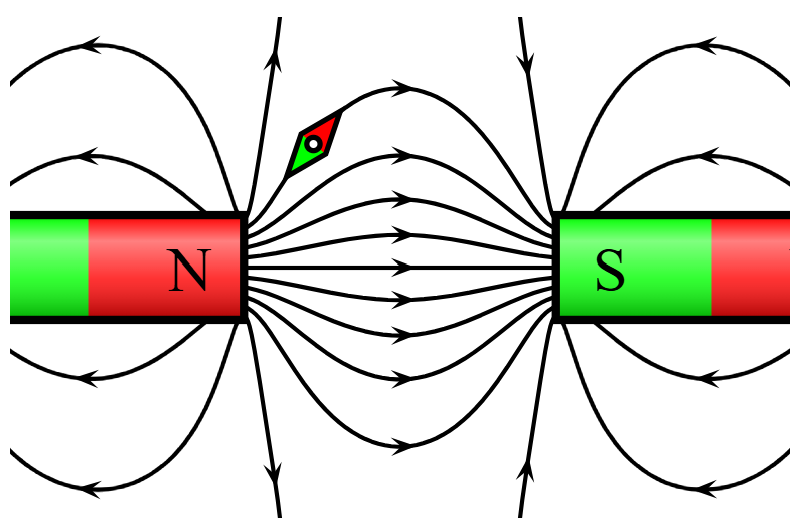
\includegraphics[width=8cm]{Bilder/zwei_magnete.png}
\end{center}
{\scriptsize Kompassnadel im Feld zwischen den einander zugewandten Polen
zweier Stabmagnete.}

Beschreiben Sie, wie sich die Kompassnadel ausrichtet, und erklären Sie
mithilfe der Feldlinien, warum.
\Antwortraum{2}
\begin{solution}
Die Kompassnadel richtet sich mit ihrem Nordpol in Richtung der
Feldlinien aus, die im Zwischenraum vom Nordpol (links) zum Südpol
(rechts) verlaufen -- ihr Nordpol zeigt also in Richtung des rechten
Magneten. Da sich die Felder beider Magnete im Zwischenraum überlagern
und dort besonders dicht sind (die beiden Magnete ziehen sich an),
schlägt die Nadel dort deutlich aus.
\end{solution}
\end{taskbox}
\end{questions}

% =============================================================================
% Vergleich: elektrisches Punktladungsfeld vs. Stabmagnetfeld
% =============================================================================
\begin{questions}
\begin{taskbox}[Vergleich: Punktladungsfeld und Stabmagnetfeld]
\question Betrachten Sie die beiden Felder nebeneinander: links das
elektrische Feld zweier entgegengesetzter Punktladungen (ein elektrischer
Dipol, bereits aus der Elektrostatik bekannt), rechts das Magnetfeld eines
Stabmagneten (ebenfalls ein Dipol).
\begin{center}
% Höhe statt Breite angeglichen: Die beiden Bilder haben sehr
% unterschiedliche Seitenverhältnisse (Punktladungsfeld breit/flach,
% Stabmagnetfeld nahezu quadratisch) -- bei gleicher Breite wirkt das
% Stabmagnetfeld dadurch fast doppelt so gross wie das Punktladungsfeld.
% Gleiche Höhe ergibt einen tatsächlich vergleichbaren visuellen Eindruck.
\begin{minipage}[t]{9.6cm}\centering
  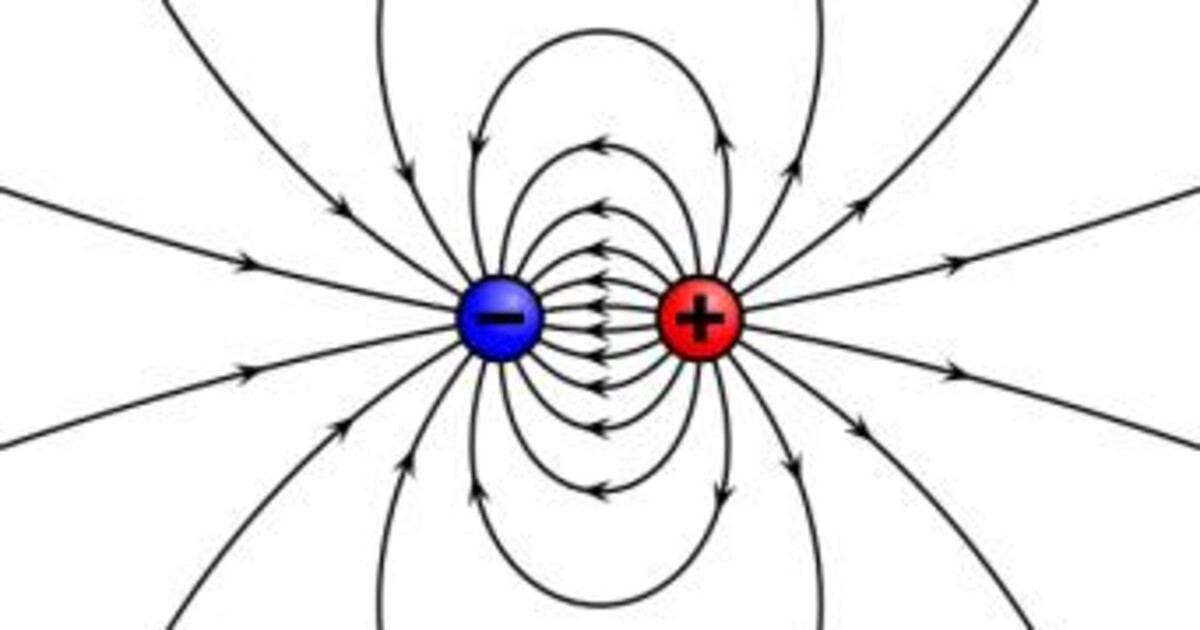
\includegraphics[height=5cm]{Bilder/elektrisches_fled_punktladungen.jpg}\\
  elektrischer Dipol
\end{minipage}\hfill
\begin{minipage}[t]{5.2cm}\centering
  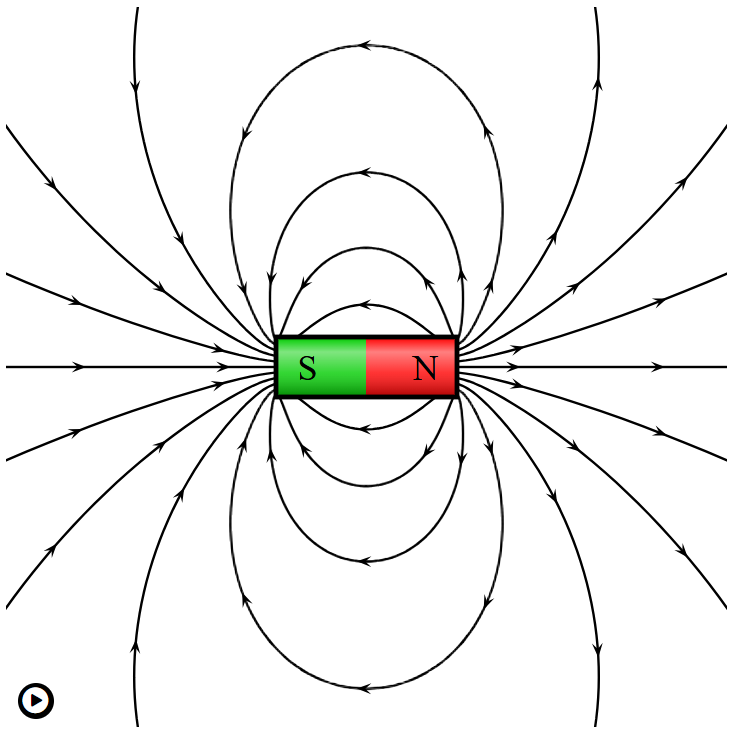
\includegraphics[height=5cm]{Bilder/magnetfeld_permanentmagnet.png}\\
  Stabmagnet
\end{minipage}
\end{center}
Beide Bilder zeigen auf den ersten Blick eine ähnliche Form. Was ist
trotzdem der wichtigste Unterschied zwischen den beiden Feldern?
\Antwortraum{3}
\begin{solution}
Die beiden Ladungen des elektrischen Dipols könnten auch für sich allein
existieren -- jede einzelne Ladung hätte dann ihr eigenes, einfaches
radiales Feld. Beim Stabmagneten ist das nicht möglich: Nord- und Südpol
lassen sich nicht voneinander trennen. Schneidet man den Magneten durch,
entstehen zwei neue, vollständige Magnete mit je einem Nord- und einem
Südpol -- nie ein isolierter einzelner Pol. Einen \glqq magnetischen
Monopol\grqq{}, das Gegenstück zu einer einzelnen elektrischen Ladung,
gibt es nicht.
\end{solution}
\end{taskbox}
\end{questions}

% =============================================================================
% Theorie: Regeln zum Zeichnen von Magnetfeldern (LZ1)
% =============================================================================
\begin{theoriebox}[Magnetfelder zeichnen]
\textbf{\emph{Regeln zum Zeichnen von Magnetfeldern:}}
\begin{itemize}[leftmargin=1.2cm,itemsep=0.2em]
  \item Feldlinien verlaufen \emph{ausserhalb} des Magneten vom Nordpol zum Südpol.
  \item Im \emph{Inneren} des Magneten schliessen sie sich vom Südpol zurück zum Nordpol -- jede Feldlinie ist eine geschlossene Kurve.
  \item Feldlinien kreuzen oder berühren sich nie.
  \item Die Richtung an einem Punkt entspricht der Richtung, in die der Nordpol einer dort platzierten Kompassnadel zeigt.
  \item Je dichter die Feldlinien gezeichnet sind, desto stärker ist das Feld an dieser Stelle.
\end{itemize}

\begin{center}
  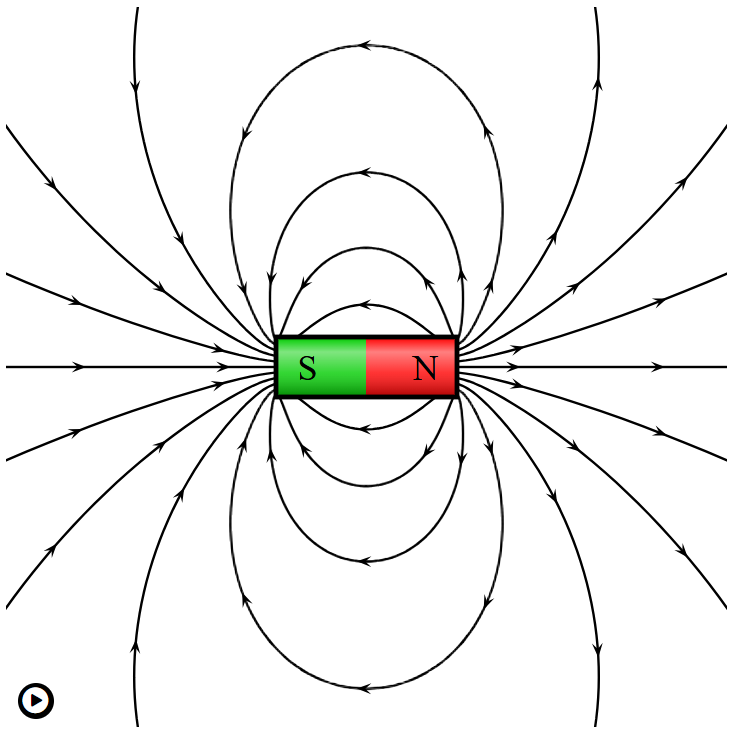
\includegraphics[height=5cm]{Bilder/magnetfeld_permanentmagnet.png}
\end{center}
{\scriptsize Nach diesen Regeln korrekt gezeichnetes Magnetfeld eines
Stabmagneten.}
\end{theoriebox}

\begin{questions}
\begin{taskbox}[Zeichenübung: Zwei Stabmagnete mit gleichnamigen Polen]
\question Zwei gleich starke Stabmagnete liegen sich gegenüber, dabei
zeigen \textbf{ihre Nordpole zueinander}. Zeichnen Sie -- unter Anwendung
der Regeln oben -- direkt in das Feld unten ein, wie die Feldlinien
zwischen und um die beiden Magnete verlaufen.
\begin{answerbox}
\vspace{4.5cm}
\begin{center}
\begin{tikzpicture}[>=Latex,scale=1]
  % linker Magnet: S (links) -- N (rechts, zeigt zur Mitte)
  \draw[thick] (-4.5,0) rectangle (-2,0.9);
  \draw[thick] (-3.25,0) -- (-3.25,0.9);
  \node at (-3.875,0.45) {S};
  \node at (-2.625,0.45) {N};
  % rechter Magnet: N (links, zeigt zur Mitte) -- S (rechts)
  \draw[thick] (2,0) rectangle (4.5,0.9);
  \draw[thick] (3.25,0) -- (3.25,0.9);
  \node at (2.625,0.45) {N};
  \node at (3.875,0.45) {S};
\end{tikzpicture}
\end{center}
\vspace{4.5cm}
\end{answerbox}
\begin{solution}
% Absichtlich FALSCHE Lösung zur Fehlersuche im Unterricht: Das Bild zeigt
% einfach die beiden unabhängigen Einzelfelder übereinandergelegt: Genau
% dadurch kreuzen sich die Feldlinien im Zwischenraum -- das ist der
% Fehler, den die Klasse finden soll (siehe Erläuterung unten).
\begin{center}
  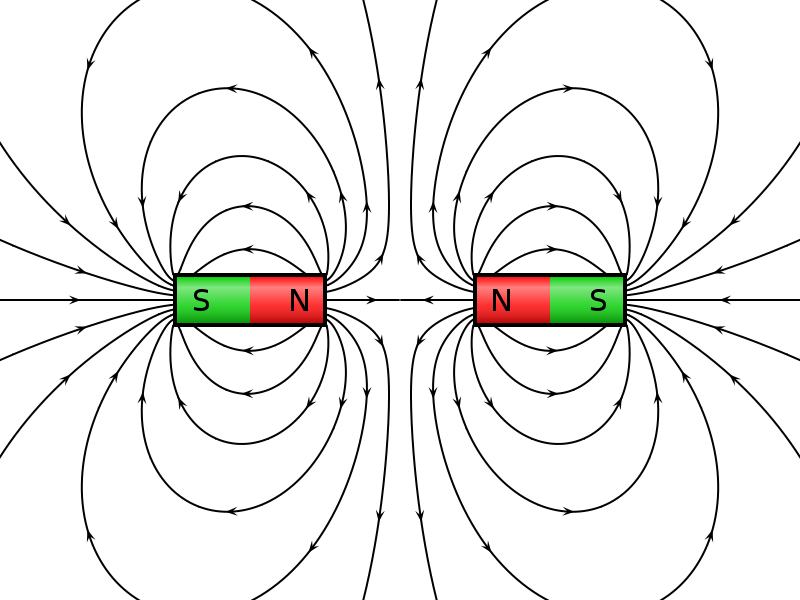
\includegraphics[width=8cm]{Bilder/Stabmagnet_gegenpolung.png}
\end{center}
\textbf{Fehlersuche:} Diese Lösung enthält absichtlich einen Fehler --
finden Sie ihn, bevor Sie weiterlesen.

Das Bild zeigt einfach die Feldlinien, die \emph{jeder Magnet für sich
allein} erzeugen würde, übereinandergelegt. Genau im Zwischenraum
\textbf{kreuzen sich} dadurch mehrere Feldlinien der beiden Magnete. Das
widerspricht der Regel, dass sich Feldlinien nie kreuzen dürfen --
ausserdem berücksichtigt das Bild gar nicht, dass sich die beiden
Magnete gegenseitig beeinflussen. Richtig ist stattdessen: Zwei
gleichnamige Pole stossen sich ab, die Feldlinien weichen im Zwischenraum
seitlich auseinander statt sich zu kreuzen, und in der Mitte entsteht ein
feldfreier Punkt (Nullstelle), an dem sich die Wirkungen beider Magnete
exakt aufheben.
\end{solution}
\end{taskbox}
\end{questions}

% =============================================================================
% Theorie: Das Erdmagnetfeld (LZ1)
% =============================================================================
\begin{theoriebox}[Das Erdmagnetfeld]
Auch die Erde selbst besitzt ein Magnetfeld, das in seiner Form demjenigen
eines riesigen Stabmagneten im Erdinneren ähnelt. Deshalb zeigt eine
Kompassnadel überall auf der Erde nach Norden.

\begin{center}
  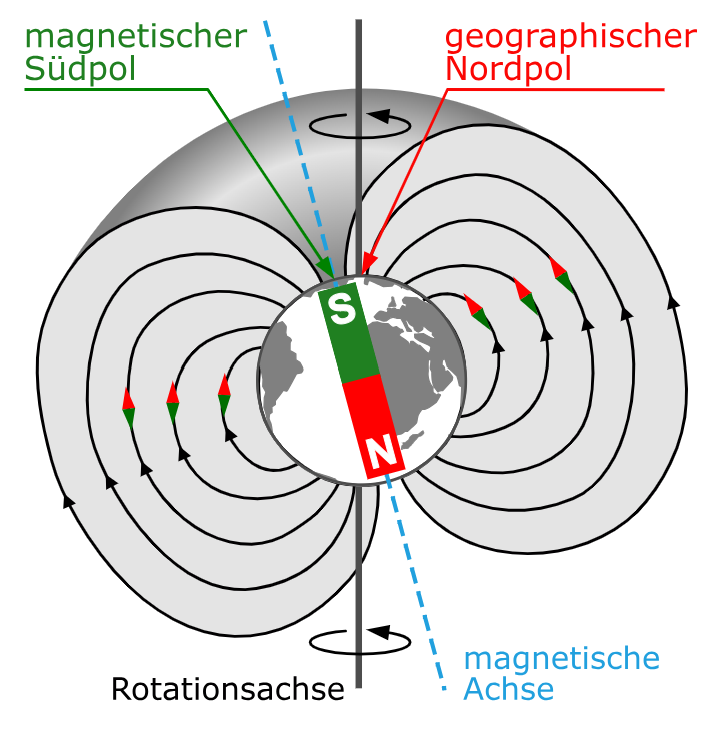
\includegraphics[width=6.5cm]{Bilder/erdmagnetfeld.png}
\end{center}
{\scriptsize Das Erdmagnetfeld: geografischer und magnetischer Nordpol
liegen nicht am selben Ort.}

\begin{hinweisbox}[Achtung, Verwechslungsgefahr]
Der \textbf{\emph{geografische Nordpol}} (die Drehachse der Erde) und der
\textbf{\emph{magnetische Nordpol}} sind \emph{nicht} derselbe Ort. Da sich
Feldlinien vom magnetischen Nordpol weg und zum magnetischen Südpol hin
bewegen, eine Kompassnadel aber am geografischen Nordpol nach Norden zeigt,
liegt dort tatsächlich der \textbf{magnetische Südpol} des Erdmagnetfelds.
\end{hinweisbox}
\end{theoriebox}

% =============================================================================
% Überleitung: Die Geschichte von Ørsted
% =============================================================================
\begin{beispielbox}[Die Geschichte von Ørsted]
\begin{center}
  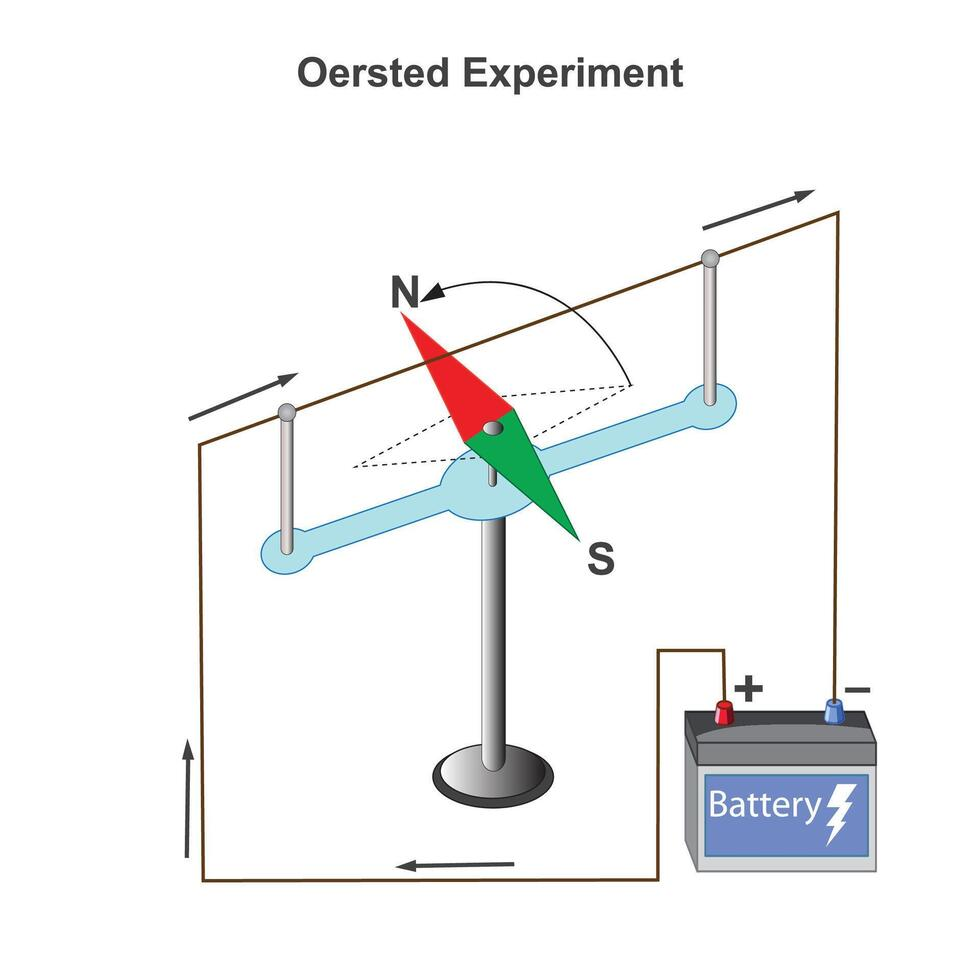
\includegraphics[width=7cm]{Bilder/oersted-experiment-showed-electric-current-creates-a-magnetic-field-fundamental-in-electromagnetism-s-development-p.jpg}
\end{center}
Im Jahr 1820 hielt der dänische Physiker Hans Christian Ørsted eine
Vorlesung, bei der zufällig eine Kompassnadel in der Nähe eines
stromdurchflossenen Drahtes lag. Als er den Stromkreis schloss, schlug die
Kompassnadel aus, obwohl niemand einen Magneten in die Nähe gebracht
hatte. Bis zu diesem Moment galten Elektrizität und Magnetismus als zwei
völlig getrennte Phänomene -- Ørsteds Zufallsbeobachtung war der erste
direkte Beweis dafür, dass fliessender Strom selbst ein Magnetfeld
erzeugt.

Genau diesen Effekt untersuchen Sie jetzt selbst.
\end{beispielbox}

% =============================================================================
% Baukasten-Experiment (Partnerarbeit): Feld bei Leiter und Spule
% =============================================================================
\begin{questions}
\begin{groupbox}[Baukasten-Experiment (Partnerarbeit): Feld bei Leiter und Spule]
% TODO: Foto des Baukastens/Versuchsaufbaus einfügen, sobald vorhanden
% (noch nicht erstellt -- keine eigene Skizze an dieser Stelle).
\question Sie erhalten einen Baukasten mit einem Stromkreis, der einen
geraden Stableiter und eine Spule enthält, sowie mehrere kleine
Kompassnadeln.
\begin{parts}
  \part[4] Untersuchen Sie mit den Kompassnadeln \textbf{beide} Bauteile
  nacheinander. Beschreiben Sie für \textbf{jedes} der beiden Felder, wie
  sich die Nadeln ausrichten: beim geraden Stableiter in verschiedenen
  Abständen rund um den Draht (wie bei Ørsted); bei der Spule innerhalb,
  an ihren beiden Enden, und seitlich davon.
  \Antwortraum{4}
  \begin{solution}
  \textbf{Gerader Leiter:} Die Kompassnadeln stellen sich tangential zu
  gedachten Kreisen um den Draht -- je näher am Draht, desto stärker der
  Ausschlag.

  \textbf{Spule:} Im Inneren zeigen alle Kompassnadeln in dieselbe
  Richtung entlang der Spulenachse (ein starkes, einheitliches Feld). An
  den beiden Enden der Spule zeigen sich deutlich erkennbare Pole: Die
  Nadeln richten sich dort wie bei einem gewöhnlichen Stabmagneten aus.
  Seitlich neben der Spule ist das Feld dagegen deutlich schwächer und
  weniger einheitlich.
  \end{solution}

  \part[3] Kehren Sie jetzt die Stromrichtung im Stromkreis um. Was
  verändert sich \textbf{sowohl} am Feld des geraden Leiters \textbf{als
  auch} am Feld der Spule?
  \Antwortraum{3}
  \begin{solution}
  \textbf{Gerader Leiter:} Die Feldrichtung kehrt sich vollständig um --
  alle Kompassnadeln um den Draht schlagen in die jeweils entgegengesetzte
  Richtung aus.

  \textbf{Spule:} Ebenfalls vollständige Umkehr -- die Kompassnadeln im
  Inneren zeigen jetzt in die Gegenrichtung, und Nord- und Südpol der
  Spule vertauschen sich.
  \end{solution}
\end{parts}
\end{groupbox}
\end{questions}

% =============================================================================
% Theorie: Rechte-Faust-Regel und Formeln (LZ2, LZ3)
% =============================================================================
\begin{theoriebox}[Das Magnetfeld des geraden Leiters]
Von oben betrachtet (Blick entlang des Drahtes) bilden die Feldlinien um
einen stromdurchflossenen, geraden Leiter \textbf{\emph{konzentrische
Kreise}}.

Die Richtung des Feldes bestimmen Sie mit der
\textbf{\emph{Rechte-Faust-Regel}}: Zeigt der Daumen der rechten Hand in
Stromrichtung, geben die gekrümmten Finger die Richtung des Magnetfelds an.

\begin{center}
  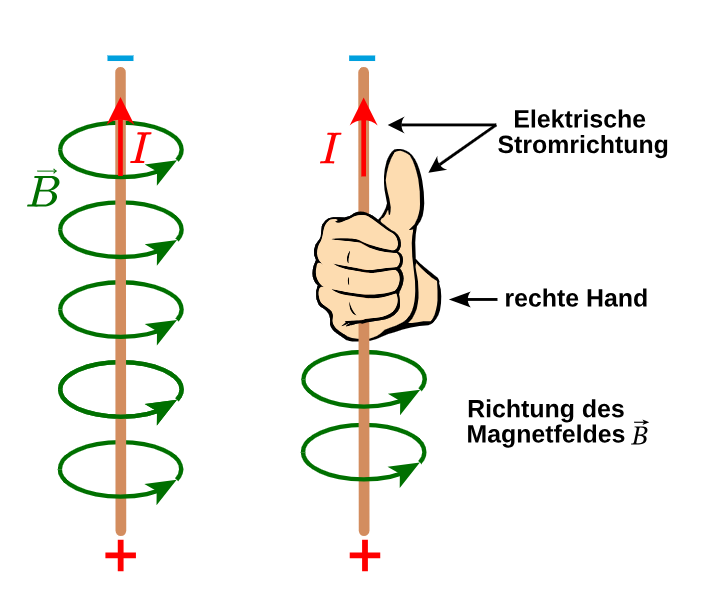
\includegraphics[width=6cm]{Bilder/leiter.png}
\end{center}
{\scriptsize Rechte-Faust-Regel für den geraden Leiter: Daumen zeigt in
Stromrichtung $I$, die gekrümmten Finger zeigen die Richtung von $\vec B$.}

Die \textbf{\emph{magnetische Flussdichte}} $B$ im Abstand $r$ von einem
geraden Leiter mit Stromstärke $I$ beträgt (ergänzen Sie die Formel und
die Einheit von $B$):
\begin{answerbox}
\vspace{0.9cm}
\hspace{1.5cm}$B = {}$\par
\vspace{0.9cm}
\end{answerbox}
\begin{solution}
\[
  B = \frac{\mu_0}{2\pi}\cdot\frac{I}{r}, \qquad \text{Einheit von } B\colon\ \si{\tesla}.
\]
Dabei ist $\mu_0$ die \textbf{\emph{magnetische Feldkonstante}}
$\mu_0 = 4\pi\cdot10^{-7}\,\si{\newton\per\ampere\squared}$, eine
Naturkonstante, die angibt, wie leicht sich ein Magnetfeld im Vakuum
aufbauen lässt.

Einheit von $B$: Aus $[\mu_0]=\si{\newton\per\ampere\squared}$ und
$[I/r]=\si{\ampere\per\meter}$ folgt (ein Faktor $\si{\ampere}$ kürzt sich
weg):
\[
  [B] = \si{\newton\per\ampere\squared}\cdot\si{\ampere\per\meter}
      = \SI{1}{\newton\per\ampere\per\meter}.
\]
Diese Einheitenkombination hat einen eigenen Namen:
\[
  \SI{1}{\newton\per\ampere\per\meter} = \text{1 Tesla} = \SI{1}{\tesla}.
\]
\end{solution}

Aus der Formel lässt sich das \textbf{\emph{Skalierungsverhalten}} direkt
ablesen: $B$ ist \textbf{\emph{proportional}} zur Stromstärke $I$ (doppelter
Strom $\to$ doppeltes Feld) und \textbf{\emph{umgekehrt proportional}} zum
Abstand $r$ (doppelter Abstand $\to$ halbes Feld).
\end{theoriebox}

\begin{theoriebox}[Das Magnetfeld der Spule]
Reiht man viele stromdurchflossene Windungen dicht aneinander, addieren
sich ihre Felder zu einem starken, im Inneren nahezu homogenen Magnetfeld
entlang der ganzen Spulenachse -- genau das haben Sie im
Baukasten-Experiment beobachtet.

\begin{center}
  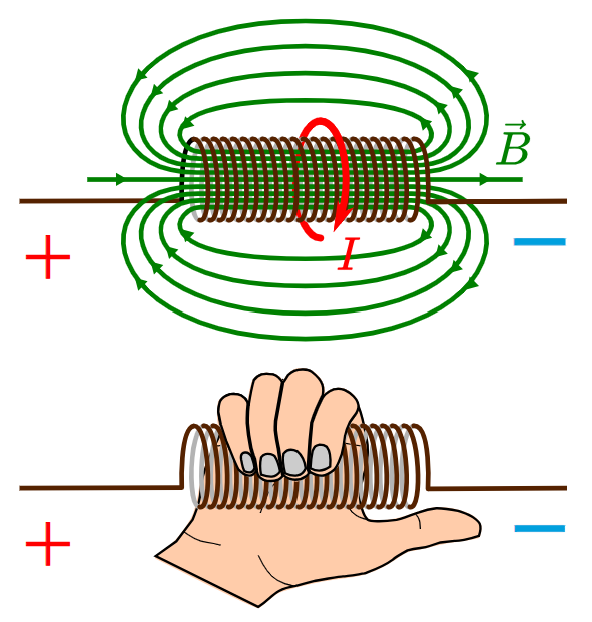
\includegraphics[width=7.5cm]{Bilder/spule.png}
\end{center}
{\scriptsize Rechte-Faust-Regel für die Spule: Zeigen die gekrümmten Finger
in Stromrichtung (Windungsrichtung), zeigt der Daumen zum Nordpol der
Spule.}

Für eine Spule mit $N$ Windungen auf der Länge $l$ gilt für die
magnetische Flussdichte im Inneren (ergänzen Sie die Formel und die
Einheit von $B$):
\begin{answerbox}
\vspace{0.9cm}
\hspace{1.5cm}$B = {}$\par
\vspace{0.9cm}
\end{answerbox}
\begin{solution}
\[
  B = \mu_0\cdot\frac{N}{l}\cdot I, \qquad \text{Einheit von } B\colon\ \si{\tesla}.
\]
($N$ ist eine reine Zahl ohne Einheit, $l$ in \si{\meter}, $I$ in
\si{\ampere}.) Den Quotienten $n=\frac{N}{l}$ (Windungen pro Meter
Spulenlänge) nennt man die \textbf{\emph{Windungsdichte}} $n$; damit lässt
sich die Formel auch kompakter schreiben als $B=\mu_0\cdot n\cdot I$.
\end{solution}
Das homogene Feld im Inneren einer Spule ist die magnetische Entsprechung
des homogenen elektrischen Feldes im Inneren eines Plattenkondensators.
\end{theoriebox}

\begin{hinweisbox}[Achtung, Verwechslungsgefahr]
Es gibt \textbf{zwei verschiedene} Rechte-Faust-Regeln: Beim
\textbf{geraden Leiter} zeigt der \textbf{Daumen} in Stromrichtung, die
\textbf{Finger} zeigen die Feldrichtung. Bei der \textbf{Spule} ist es
umgekehrt: Die \textbf{Finger} zeigen in Stromrichtung (Windungsrichtung),
der \textbf{Daumen} zeigt zum Nordpol. Prüfen Sie bei jeder Aufgabe zuerst,
um welchen Fall es sich handelt.
\end{hinweisbox}

\end{document}
